%
% Copyright 2018 Joel Feldman, Andrew Rechnitzer and Elyse Yeager.
% This work is licensed under a Creative Commons Attribution-NonCommercial-ShareAlike 4.0 International License.
% https://creativecommons.org/licenses/by-nc-sa/4.0/
%
\questionheader{ex:s2.11}



%%%%%%%%%%%%%%%%%%
\subsection*{\Conceptual}
%%%%%%%%%%%%%%%%%%


\begin{question}
If we implicitly differentiate $x^2+y^2=1$, we get the equation $2x+2yy'=0$. In the step where we differentiate $y^2$ to obtain $2yy'$, which rule(s) below are we using?
\begin{center}
(a) power rule \qquad (b) chain rule \qquad
 (c) quotient rule \\(d) derivatives of exponential functions
\end{center}
\end{question}
\begin{hint}
Where did the $y'$ come from?
\end{hint}
\begin{answer}
(a) and (b)
\end{answer}
\begin{solution}
We use the power rule (a) and the chain rule (b): the power rule tells us to ``bring down the 2", and the chain rule tells us to multiply by $y'$. \medskip

There is no need for the quotient rule here, as there are no quotients. Exponential functions have the form $(\mbox{constant})^{\mbox{function}}$, but our function has the form $(\mbox{function})^{\mbox{constant}}$, so we did not use (d).
\end{solution}

\begin{Mquestion}
Using the picture below, estimate $\ds\diff{y}{x}$ at the three points where the curve crosses the $y$-axis.
\begin{center}
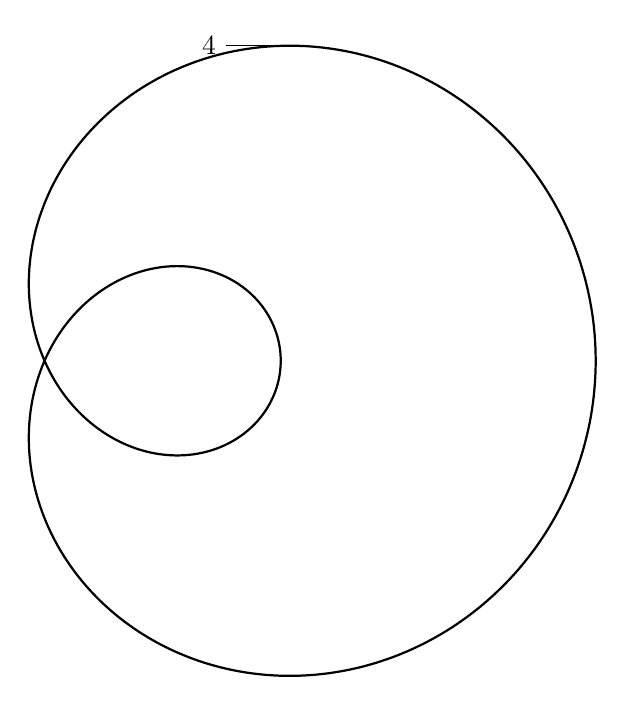
\begin{tikzpicture}
\YEaxis{4.5}{4.5}
\foreach\x in {1,...,4}{\YExcoord{\x}{\x}}
\foreach\x in {1,...,3}{\YEycoord{\x}{\x}}
\draw (.2,4)--(-.7,4) node[left]{4};
\foreach\x in {-4,-3,-2,-1}{\YExcoord{\x}{\x}}
\foreach\x in {-4,-3,-2,-1}{\YEycoord{\x}{\x}}
\draw[shift={(-3,0)}, rotate=90 ] [thick, domain=0:2*pi, samples=200, smooth]
  plot (xy polar cs:angle={\x r}, radius={2-5*sin(\x r)});
\end{tikzpicture}
\end{center}
Remark: for this curve, one value of $x$ may correspond to multiple values of $y$. So, we cannot express this curve as $y=f(x)$ for any function $x$. This is one typical situation where we might use implicit differentiation.
\end{Mquestion}
\begin{hint}
The three points to look at are $(0,-4)$, $(0,0)$, and $(0,4)$. What does the slope of the tangent line look like there?
\end{hint}
\begin{answer}
At $(0,4)$ and $(0,-4)$, $\ds\diff{y}{x}$ is 0; at $(0,0)$, $\ds\diff{y}{x}$ does not exist.
\end{answer}
\begin{solution}
At $(0,4)$ and $(0,-4)$, the curve looks to be horizontal, if you zoom in: a tangent line here would have derivative zero. At the origin, the curve looks like its tangent line is vertical, so $\ds\diff{y}{x}$ does not exist.

\begin{center}
\begin{tikzpicture}
\YEaxis{4.5}{4.5}
\draw[shift={(-3,0)}, rotate=90 ,thick] [domain=0:2*pi, samples=100]
  plot (xy polar cs:angle={\x r}, radius={2-5*sin(\x r)});
  \color{red};
  \draw[thick, dashed] (2,4)--(-2,4);
    \draw[thick, dashed] (2,-4)--(-2,-4);
      \draw[ultra thick, dashed] (0.05,-1.5)--(0.05,1.5);
     \draw (0,0) node[vertex]{};
         \draw (0,4) node[vertex]{};
             \draw (0,-4) node[vertex]{};
\end{tikzpicture}
\end{center}
\end{solution}
%%%%%add in tangent lines to pic

\begin{question}
Consider the unit circle, formed by all points $(x,y)$ that satisfy $x^2+y^2=1$.
\begin{center}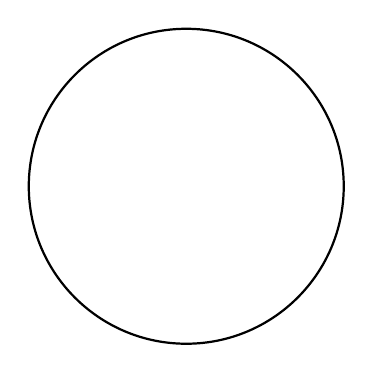
\begin{tikzpicture}
\YEaxis{2.5}{2.5}
\draw[thick] node[shape=circle, minimum size=4cm, inner sep=0, draw]{};
\end{tikzpicture}\end{center}
\begin{enumerate}[(a)]
\item Is there a function $f(x)$ so that $y=f(x)$ completely describes the unit circle? That is, so that the points $(x,y)$ that make the equation $y=f(x)$ true are exactly the same points that make the equation $x^2+y^2=1$ true?
\item Is there a function $f'(x)$ so that $y=f'(x)$ completely describes the slope of the unit circle? That is, so that for every point $(x,y)$ on the unit circle, the slope of the tangent line to the circle at that point is given by $f'(x)$?
\item Use implicit differentiation to find an expression for $\ds\diff{y}{x}$. Simplify until the expression is a function in terms of $x$ only (not $y$), or explain why this is impossible.
\end{enumerate}
\end{question}
\begin{hint} A function must pass the vertical line test: one input \emph{cannot} result in two different outputs.
\end{hint}
\begin{answer}
(a) no \qquad (b) no\\
$\ds\diff{y}{x}=-\dfrac{x}{y}$. It is not possible to write $\ds\diff{y}{x}$ as a function of $x$, because (as stated in (b)) one value of $x$ may give two values of $\ds\diff{y}{x}$. For instance, when $x=\pi/4$, at the point $\left(\dfrac{\pi}{4},\dfrac{1}{\sqrt{2}}\right)$ the circle has slope $\ds\diff{y}{x}=-1$, while
at the point $\left(\dfrac{\pi}{4},\dfrac{-1}{\sqrt{2}}\right)$ the circle has slope $\ds\diff{y}{x}=1$.
\end{answer}
\begin{solution}
(a) No. A function must pass the vertical line test: one input cannot result in two (or more) outputs. Since one value of $x$ sometimes corresponds to two values of $y$ (for example, when $x=\pi/4$, $y$ is $\pm 1/\sqrt{2}$), there is no function $f(x)$ so that $y=f(x)$ captures every point on the circle.

Remark: $y=\pm\sqrt{1-x^2}$ does capture every point on the unit circle. However, since one input $x$ sometimes results in two outputs $y$, this expression is not a function.

(b) No, for the same reasons as (a). If $f'(x)$ is a function, then it can give at most one slope corresponding to one value of $x$.
Since one value of $x$ can correspond to two points on the circle with different slopes, $f'(x)$ cannot give the slope of every point on the circle.
For example, fix any $0<a<1$. There are two points
         on the circle with $x$-coordinate equal to $a$. At the upper one, the slope
         is strictly negative. At the lower one, the slope is
         strictly positive.

(c) We differentiate:
\begin{align*}
2x+2y\diff{y}{x}&=0
\intertext{and solve for $\ds\diff{y}{x}$}
\diff{y}{x}&=-\frac{x}{y}
\end{align*}
But there is a $y$ in the right-hand side of this equation, and it's not clear how to get it out. Our answer in (b) tells us that, actually, we \emph{can't} get it out, if we want the right-hand side to be a function of $x$. The derivative cannot be expressed as a function of $x$, because one value of $x$ corresponds to multiple points on the circle.

Remark: since $y=\pm\sqrt{1-x^2}$, we could try writing
\[\diff{y}{x}=-\frac{x}{y}=\pm\frac{x}{\sqrt{1-x^2}}\]
but this is not a \emph{function} of $x$. Again, in a function, one input leads to at most one output, but here one value of $x$ will usually lead to two values of $\diff{y}{x}$.
\end{solution}




%%%%%%%%%%%%%%%%%%
\subsection*{\Procedural}
%%%%%%%%%%%%%%%%%%


\begin{Mquestion}[2009H]
Find $\ds\diff{y}{x}$ if $xy + e^x + e^y = 1$.
\end{Mquestion}
\begin{hint} Remember that $y$ is a function of $x$.
Use implicit differentiation, then collect all the terms containing $\ds\diff{y}{x}$ on one side of the equation to solve for $\ds\diff{y}{x}$.
\end{hint}
\begin{answer}
$\ds\diff{y}{x}=-\dfrac{e^x+y}{e^y+x}$
\end{answer}
\begin{solution} Remember that $y$ is a function of $x$.
We begin with implicit differentiation.
\begin{align*}
xy + e^x + e^y &= 1\\
y+x\diff{y}{x}+e^x+e^y\diff{y}{x}&=0
\intertext{Now, we solve for $\ds\diff{y}{x}$.}
x\diff{y}{x}+e^y\diff{y}{x}&=-(e^x+y)\\
(x+e^y)\diff{y}{x}&=-(e^x+y)\\
\diff{y}{x}&=-\frac{e^x+y}{e^y+x}
\end{align*}
\end{solution}



\begin{question}[2015Q]
If $e^y=xy^2+x$, compute $\ds\diff{y}{x}$.
\end{question}
\begin{hint} Differentiate implicitly, then solve for $y'$.
\end{hint}
\begin{answer} $\ds\diff{y}{x} = \dfrac{y^2+1}{e^y-2xy}$
\end{answer}
\begin{solution} Differentiate both sides of the equation with respect to $x$:
\begin{align*}
e^y\diff{y}{x}&=x\cdot2y\diff{y}{x}+y^2+1
\intertext{Now, get the derivative on one side and solve}
e^y\diff{y}{x}-2xy\diff{y}{x}&=y^2+1\\
\diff{y}{x}\left(e^y-2xy\right)&=y^2+1\\
\diff{y}{x}&=\frac{y^2+1}{e^y-2xy}
\end{align*}
\end{solution}



\begin{Mquestion}[2015Q]
If $x^2\tan(\pi y/4)+2x\log(y) = 16$, then find $y'$ at the points where $y=1$.
\end{Mquestion}
\begin{hint}
Remember that $y$ is a function of $x$. You can determine
        explicitly the values of $x$ for which $y(x)=1$.
\end{hint}
\begin{answer}
At $(x,y)=(4,1)$, $y' =
-\dfrac{1}{\pi + 1}$.
At $(x,y)=(-4,1)$,  $y' = \dfrac{1}{\pi-1}$.
\end{answer}
\begin{solution}
\begin{itemize}
 \item First we find the $x$-coordinates where $y=1$.
\begin{align*}
  x^2\tan\left(\frac{\pi}{4}\right)+2x\log(1) &= 16 \\
  x^2\cdot 1 +2x\cdot 0 &=16\\
  x^2 &= 16\\
\end{align*}
So $x=\pm 4$.
\item Now we use implicit differentiation to get $y'$ in terms of $x,y$:
\begin{align*}
  x^2\tan(\pi y/4)+2x\log(y) &= 16\\
  2x\tan(\pi y/4) + x^2 \frac{\pi}{4}\sec^2(\pi y/4)\cdot y' + 2\log(y) + \frac{2x}{y} \cdot y' &= 0\,.\\
\end{align*}
\item Now set $y=1$ and use $\tan(\pi/4)=1\,, \sec(\pi/4)=\sqrt{2}$ to get
\begin{align*}
  2x\tan(\pi/4) + x^2 \frac{\pi}{4} \sec^2(\pi/4)y' + 2\log(1) + 2x\cdot y' &= 0\\
  2x + \frac{\pi}{2} x^2 y' +2x y' &= 0 \\
  y' = -\frac{2x}{x^2 \pi/2 + 2x} &= -\frac{4}{\pi x + 4}  \\
\end{align*}
\item So at $(x,y)=(4,1)$ we have $y' = -\dfrac{4}{4\pi+4} =
-\dfrac{1}{\pi + 1}$
\item and at $(x,y)=(-4,1)$ we have $y' = \dfrac{1}{\pi-1}$
\end{itemize}
\end{solution}


\begin{Mquestion}[2015Q]
 If $x^3+y^4 = \cos(x^2+y)$ compute $\diff{y}{x}$.
\end{Mquestion}
\begin{answer}
$ -\ds\frac{2x\sin(x^2+y)+3x^2}{4y^3+\sin(x^2+y)}$
\end{answer}
\begin{solution}
Differentiate the equation and solve:
\begin{align*}
  3x^2 + 4y^3 \diff{y}{x} &= -\sin(x^2+y) \cdot\left(2x + \diff{y}{x}\right) \\
  \diff{y}{x} &= -\frac{2x\sin(x^2+y)+3x^2}{4y^3+\sin(x^2+y)}
\end{align*}
\end{solution}

\begin{question}[2015Q]
If $x^2e^y + 4x\cos(y) = 5$, then find $y'$ at the points where $y=0$.
\end{question}
\begin{hint} Plug in $y=0$ at a strategic point in your work to simplify your computation.
\end{hint}
\begin{answer}
At $(x,y)=(1,0)$,  $y' = -6$,
and at $(x,y)=(-5,0)$,  $y' = \frac{6}{25}$.
\end{answer}
\begin{solution}
\begin{itemize}
 \item First we find the $x$-coordinates where $y=0$.
\begin{align*}
  x^2e^0+4x\cos(0) &= 5 \\
  x^2 +4x - 5 &=0\\
  (x+5)(x-1)&=0
\end{align*}
So $x=1,-5$.
\item Now we use implicit differentiation to get $y'$ in terms of $x,y$:
\begin{align*}
  x^2e^y+4x\cos(y) &= 5 & \text{differentiate both sides} \\
  x^2 \cdot e^y \cdot y' + 2x e^y + 4x(-\sin(y)) \cdot y' + 4\cos(y) &= 0
\end{align*}
\item Now set $y=0$ to get
\begin{align*}
  x^2 \cdot e^0 \cdot y' + 2x e^0 + 4x(-\sin(0)) \cdot y' + 4\cos(0) &= 0  \\
  x^2y' + 2x  + 4 &=0 \\
  y' &= - \frac{4+2x}{x^2}.
\end{align*}
\item So at $(x,y)=(1,0)$ we have $y' = -6$,
\item and at $(x,y)=(-5,0)$ we have $y' = \frac{6}{25}$.
\end{itemize}
\end{solution}


\begin{question}[2015Q]
If $x^2+y^2 = \sin(x+y)$ compute $\diff{y}{x}$.
\end{question}
\begin{answer}
$\diff{y}{x} = \dfrac{\cos(x+y)-2x}{2y-\cos(x+y)}$
\end{answer}
\begin{solution}
 Differentiate the equation  and solve:
\begin{align*}
  2x + 2y \diff{y}{x} &= \cos(x+y) \cdot\left(1 + \diff{y}{x}\right) \\
  \diff{y}{x} &= \frac{\cos(x+y)-2x}{2y-\cos(x+y)}
\end{align*}
\end{solution}


\begin{question}[2015Q]
If $x^2\cos(y)+2xe^y = 8$, then find $y'$ at the points where $y=0$.
\end{question}
\begin{hint} Plug in $y = 0$ at a strategic point in your work to
        simplify your computation.
       \end{hint}
\begin{answer}
At $(x,y)=(2,0)$ we have $y' = -\frac{3}{2}$,
 and at $(x,y)=(-4,0)$ we have $y' = -\frac{3}{4}$.
\end{answer}
\begin{solution}
\begin{itemize}
 \item First we find the $x$-coordinates where $y=0$.
\begin{align*}
  x^2\cos(0)+2xe^0 &= 8 \\
  x^2 +2x - 8 &=0\\
  (x+4)(x-2)&=0
\end{align*}
So $x=2,-4$.
\item Now we use implicit differentiation to get $y'$ in terms of $x,y$:
\begin{align*}
  x^2\cos(y)+2xe^y &= 8 & \text{differentiate both sides} \\
  x^2 \cdot (-\sin y) \cdot y' + 2x \cos y + 2xe^y \cdot y' + 2e^y &= 0
\end{align*}
\item Now set $y=0$ to get
\begin{align*}
  x^2 \cdot (-\sin 0) \cdot y' + 2x \cos 0 + 2xe^0 \cdot y' + 2e^0 &= 0  \\
  0 + 2x + 2xy' + 2 &=0 \\
  y' &= - \frac{2+2x}{2x} = -\frac{1+x}{x}
\end{align*}
\item So at $(x,y)=(2,0)$ we have $y' = -\frac{3}{2}$,
\item and at $(x,y)=(-4,0)$ we have $y' = -\frac{3}{4}$.
\end{itemize}
\end{solution}


\begin{Mquestion}
At what points on the ellipse $x^2+3y^2=1$ is the tangent line parallel to the line $y=x$?
\end{Mquestion}
\begin{hint}
If the tangent line has slope $y'$, and it is parallel to $y=x$, then $y'=1$.
\end{hint}
\begin{answer}
$\left(\dfrac{\sqrt{3}}{2},\dfrac{-1}{2\sqrt{3}}\right)$,
$\left(\dfrac{-\sqrt{3}}{2},\dfrac{1}{2\sqrt{3}}\right)$
\end{answer}
\begin{solution}
The question asks at which points on the ellipse $\ds\diff{y}x{}=1$. So, we begin by differentiating, implicitly:
\begin{align*}
2x+6y\diff{y}{x}&=0
\intertext{We could solve for $\ds\diff{y}{x}$ at this point, but it's not necessary. We want to know when $\ds\diff{y}{x}$ is equal to one:}
2x+6y(1)&=0\\
x&=-3y
\intertext{That is, $\ds\diff{y}{x}=1$ at those points along the ellipse where $x=-3y$. We plug this into the equation of the ellipse to find the coordinates of these points.}
\left(-3y\right)^2+3y^2&=1\\
12y^2&=1\\
y=\pm\frac{1}{\sqrt{12}}=\pm\frac{1}{2\sqrt{3}}
\end{align*}
So, the points along the ellipse where the tangent line is parallel to the line $y=x$ occur when $y=\dfrac{1}{2\sqrt{3}}$ and $x=-3y$, and when $y=\dfrac{-1}{2\sqrt{3}}$ and $x=-3y$. That is, the points $\left(\dfrac{-\sqrt{3}}{2},\dfrac{1}{2\sqrt{3}}\right)$ and
$\left(\dfrac{\sqrt{3}}{2},\dfrac{-1}{2\sqrt{3}}\right)$.
\end{solution}


\begin{question}[2007H]
 For the curve defined by the equation
$\sqrt{xy} = x^2y-2$, find the slope of the tangent
line at the point $(1, 4)$.
\end{question}
\begin{hint}
You don't need to solve for $y'$ in general: only at a single point.
\end{hint}
\begin{answer}
$-\dfrac{28}{3}$
\end{answer}
\begin{solution}
First, we differentiate implicitly with respect to $x$.
\begin{align*}
\sqrt{xy} &= x^2y-2\\
\frac{1}{2\sqrt{xy}}\cdot \diff{}{x}\{xy\}&=(2x)y+x^2\ds\diff{y}{x}\\
\frac{y+x\diff{y}{x}}{2\sqrt{xy}}&=2xy+x^2\diff{y}{x}
\intertext{Now, we plug in $x=1$, $y=4$, and solve for $\ds\diff{y}{x}$:}
\frac{4+\diff{y}{x}}{4}&=8+\diff{y}{x}\\
\diff{y}{x}&=-\frac{28}{3}
\end{align*}
\end{solution}



\begin{question}[2006H]
If $x^2y^2+x\sin(y)=4$, find $\ds\diff{y}{x}$.
\end{question}
\begin{hint} After you differentiate implicitly, get all the terms containing $y'$ onto one side so you can solve for $y'$.
\end{hint}
\begin{answer}
$\ds\diff{y}{x}=-\dfrac{2xy^2+\sin y}{2x^2y+x\cos y}$
\end{answer}
\begin{solution}
Implicitly differentiating $x^2y(x)^2+x\sin(y(x))=4$ with respect to $x$
gives
\begin{align*}
2xy^2&+2x^2yy'+\sin y+xy'\cos y=0
\intertext{Then we gather the terms containing $y'$ on one side, so we can solve for $y'$:}
2x^2yy'&+xy'\cos y=-2xy^2-\sin y\\
y'(2x^2y&+x\cos y)=-2xy^2-\sin y\\
 y'&=-\frac{2xy^2+\sin y}{2x^2y+x\cos y}
\end{align*}
\end{solution}

%%%%%%%%%%%%%%%%%%
\subsection*{\Application}
%%%%%%%%%%%%%%%%%%


\begin{question}[2015Q]If $x^2+(y+1)e^y = 5$, then find $y'$ at the points where $y=0$.
\end{question}
\begin{hint} You don't need to solve for $\diff{y}{x}$ for all values of $x$--only when $y=0$.
\end{hint}
\begin{answer} At $(x,y)=(2,0)$, $y' = -2$. At  $(x,y)=(-2,0)$,  $y' = 2$.
\end{answer}
\begin{solution}
\begin{itemize}
 \item First we find the $x$-ordinates where $y=0$.
\begin{align*}
  x^2+(1)e^0 &= 5 \\
  x^2 +1 &=5\\
  x^2&=4
\end{align*}
So $x=2,-2$.
\item Now we use implicit differentiation to get $y'$ in terms of $x,y$:
\begin{align*}
2x+(y+1)e^y\diff{y}{x}+e^y\diff{y}{x}&=0
\end{align*}
\item Now set $y=0$ to get
\begin{align*}
2x+(0+1)e^0\diff{y}{x}+e^0\diff{y}{x}&=0\\
2x+\diff{y}{x}+\diff{y}{x}&=0\\
2x&=-2\diff{y}{x}\\
x&=-\diff{y}{x}
\end{align*}
\item So at $(x,y)=(2,0)$ we have $y' = -2$,
\item and at $(x,y)=(-2,0)$ we have $y' = 2$.
\end{itemize}
\end{solution}



\begin{question}
For what values of $x$ do the circle $x^2+y^2=1$ and the ellipse $x^2+3y^2=1$ have parallel tangent lines?
\end{question}
\begin{hint}
\end{hint}
\begin{answer} $x=0$, $x=1$, $x=-1$
\end{answer}
\begin{solution}
The slope of the tangent line is, of course, given by the derivative, so let's start by finding $\diff{y}{x}$ of both shapes.
\begin{align*}
\intertext{For the circle, we differentiate implicitly}
2x+2y\diff{y}{x}&=0
\intertext{and solve for $\ds\diff{y}{x}$}
\diff{y}{x}&=-\frac{x}{y}
\intertext{For the ellipse, we also differentiate implicitly:}
2x+6y\diff{y}{x}&=0
\intertext{and solve for $\ds\diff{y}{x}$}
\diff{y}{x}&=-\frac{x}{3y}
\intertext{What we want is a value of $x$ where both derivatives are equal. However, they might have different values of $y$, so let's let $y_1$ be the $y$-values associated with $x$ on the circle, and let $y_2$ be the $y$-values associated with $x$ on the ellipse.
That is, $x^2+ y_1^2=1$ and $x^2+3y_2^2=1$. For the slopes
             at $(x,y_1)$ on the circle and $(x,y_2)$ on the ellipse to
             be equal, we need:}
-\frac{x}{y_1}&=-\frac{x}{3y_2}\\
x\left(\frac{1}{y_1}-\frac{1}{3y_2}\right)&=0
\intertext{So $x=0$ or $y_1=3y_2$. Let's think about which $x$-values will have a $y$-coordinate of the circle be three times as large as a $y$-coordinate of the ellipse. If $y_1=3y_2$,  $(x,y_1)$ is on the circle, and $(x,y_2)$ is on the ellipse, then
$x^2+y_1^2 =x^2+(3y_2)^2=1$ and $x^2+3y_2^2=1$. In this case:}
x^2+9y_2^2&=x^2+3y_2^2\\
9y_2^2&=3y_2^2\\
y_2&=0\\
x&=\pm 1
\end{align*}
We need to be a tiny bit careful here: when $y=0$, $y'$ is not defined for either curve. For both curves, when $y=0$, the tangent lines are vertical (and so have no real-valued slope!). Two vertical lines are indeed parallel.

So, for $x=0$ and for $x=\pm1$, the two curves have parallel tangent lines.
\begin{center}\begin{tikzpicture}
\YEaxis{4}{4};
\draw[thick] plot[domain=-3:3, samples=100](\x,{sqrt(9-\x*\x)});
\draw[thick] plot[domain=-3:3, samples=100](\x,{-sqrt(9-\x*\x)});
\draw (.5,-3) node[below right]{$x^2+y^2=1$};

\draw[thick, blue] plot[domain=-3:3, samples=100](\x,{sqrt(3-\x*\x/3)});
\draw[thick, blue] plot[domain=-3:3, samples=100](\x,{-sqrt(3-\x*\x/3)});
\draw[blue] (2,1) node[above right]{$x^2+3y^2=1$};

\color{red}
\draw (3,0) node[vertex]{};
\draw[thick, dashed] (3,-1)--(3,1);
\draw (-3,0) node[vertex]{};
\draw[thick, dashed] (-3,-1)--(-3,1);
\draw (0,1.73) node[vertex]{};
\draw[thick, dashed] (-1,1.73)--(1,1.73);
\draw (0,-1.73) node[vertex]{};
\draw[thick, dashed] (-1,-1.73)--(1,-1.73);
\draw (0,3) node[vertex]{};
\draw[thick, dashed] (-1,3)--(1,3);
\draw (0,-3) node[vertex]{};
\draw[thick, dashed] (-1,-3)--(1,-3);
\end{tikzpicture}\end{center}
\end{solution}
